\documentclass[e4_tp1_main.tex]{subfiles}
\begin{document}

\section{Disparo de un transistor MOSFET}

Para el circuito de disparo propuesto se utilizó un valor de $V_{gg}=10V$, y los datos del transistor se fueron obteniendo de la hoja de datos del IRF530 provista por Vishay, como se irá mostrando en el desarrollo.

\begin{figure}[H]
\centering
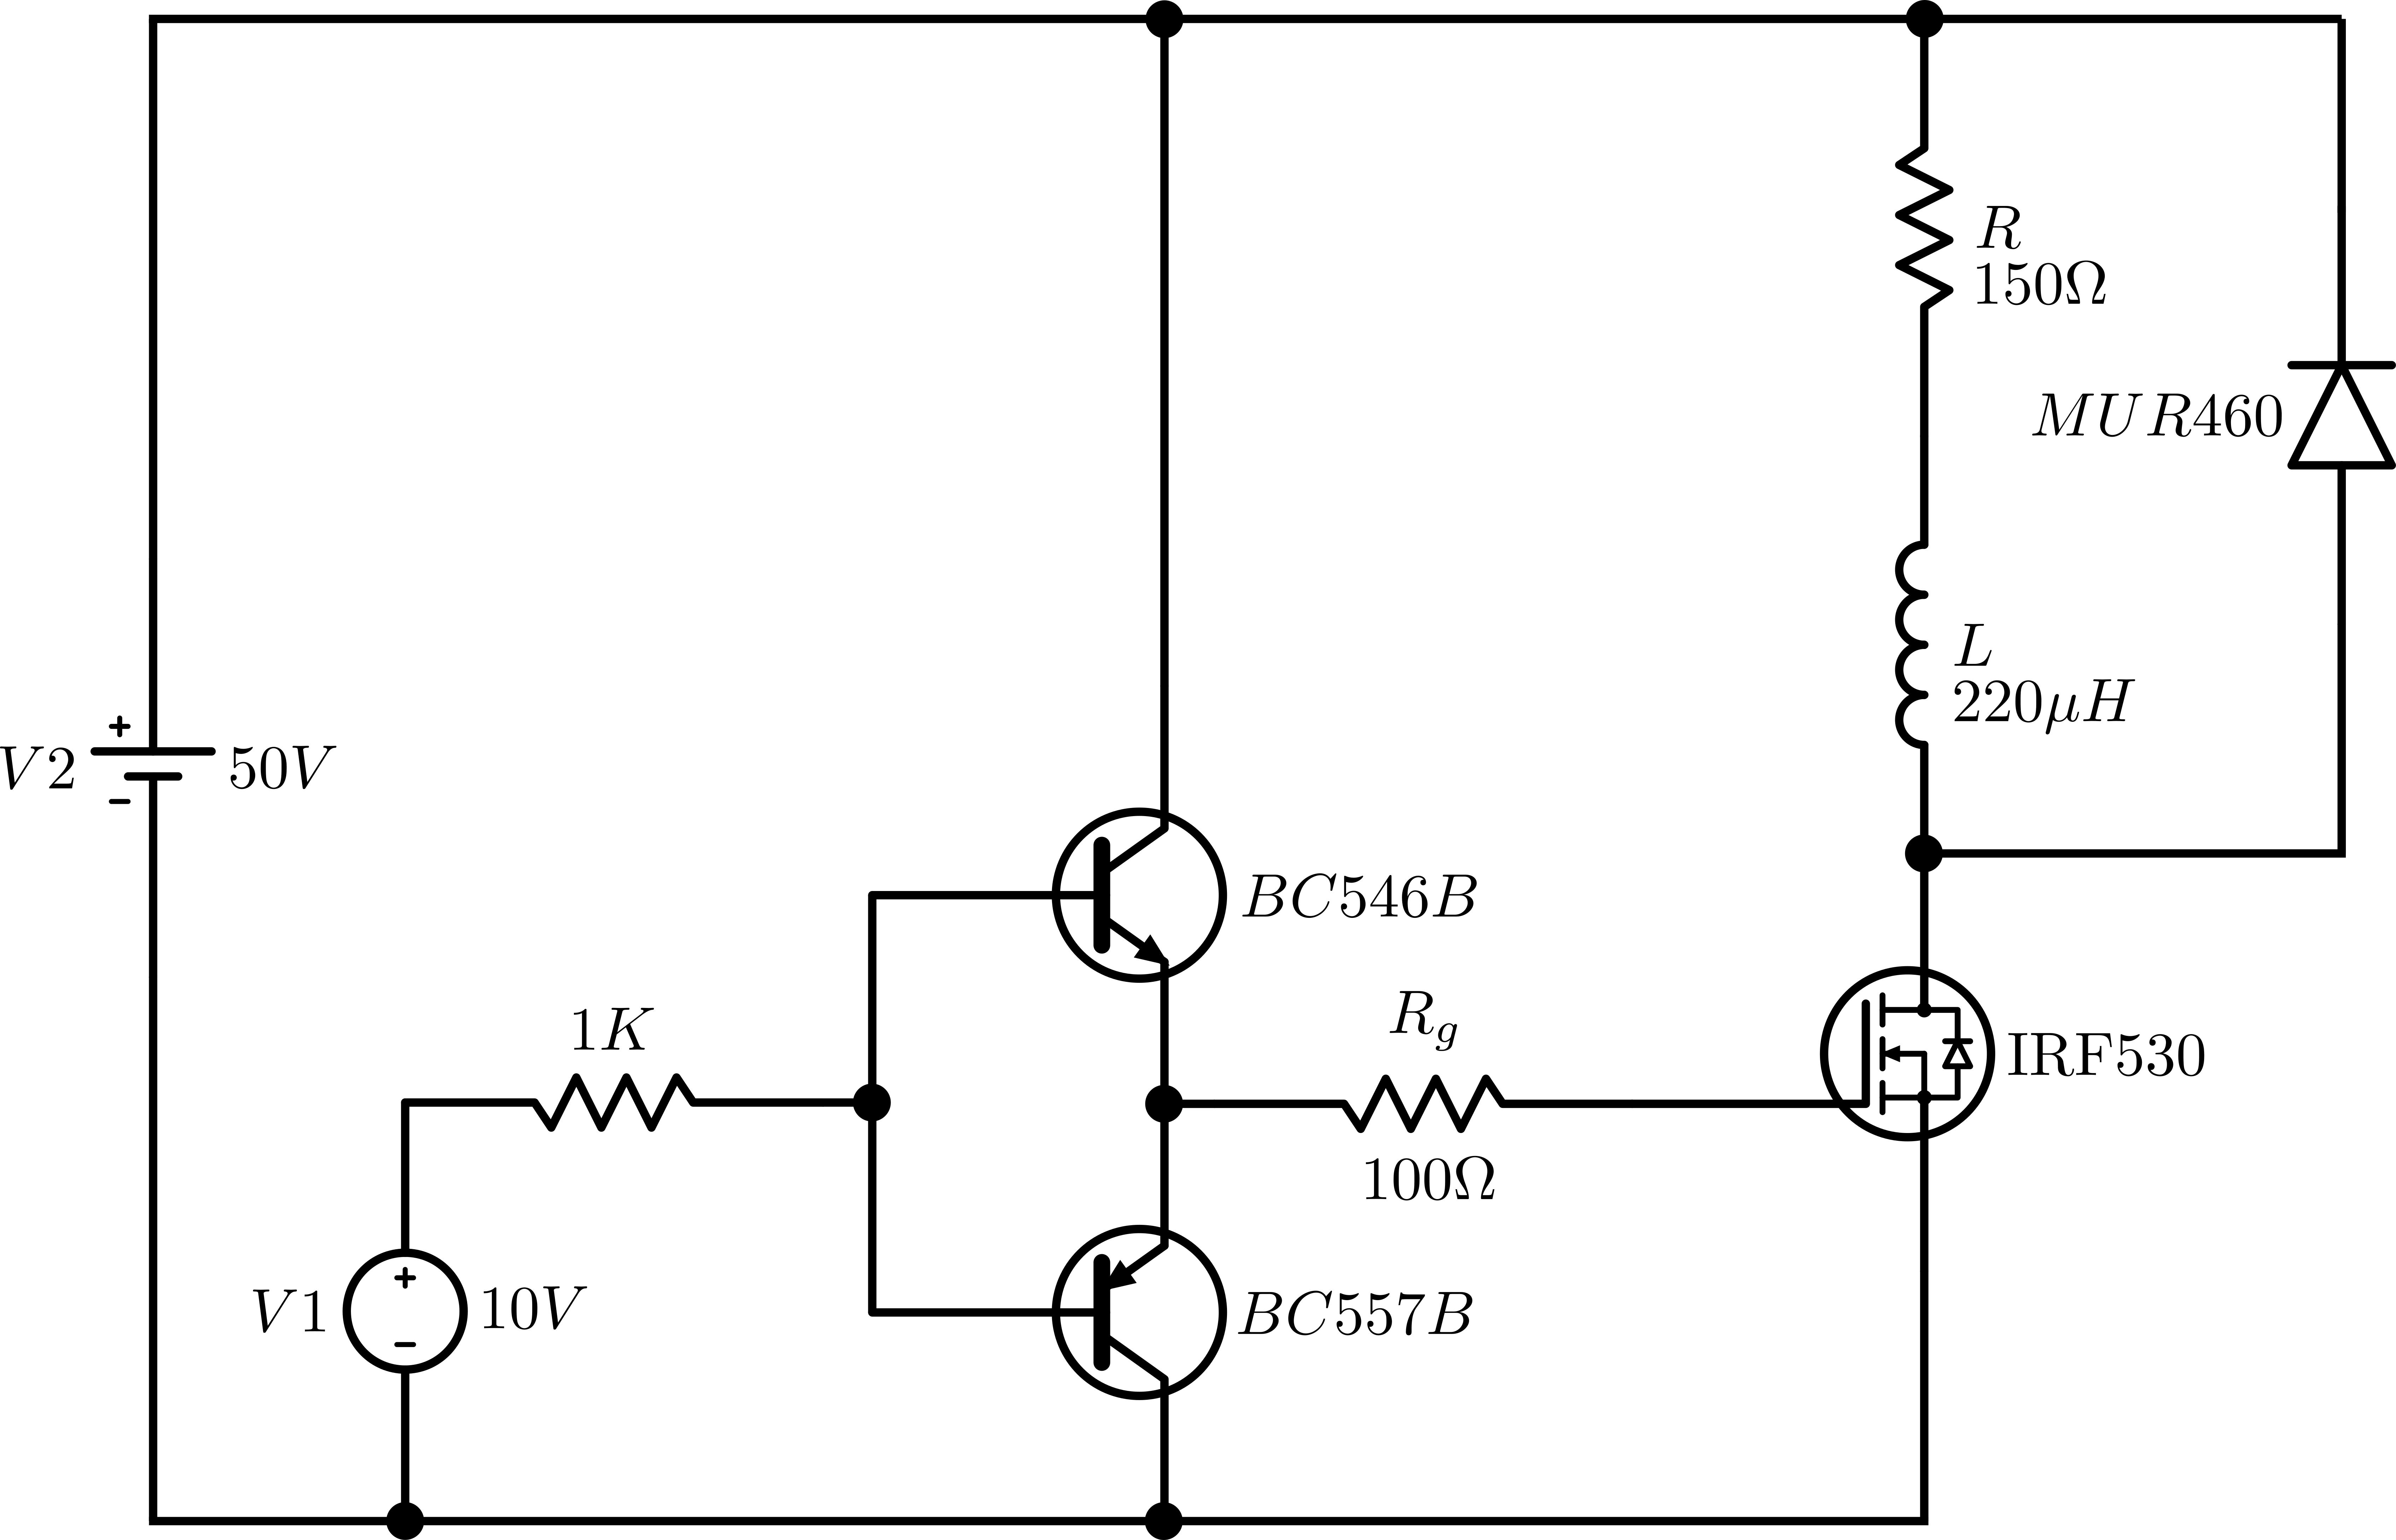
\includegraphics[width=0.7\linewidth]{Imagenes/Punto1/CircuitoDisparo.png}
\end{figure}

\subsection*{a) Cálculo teórico de los tiempos de conmutación}

Para el momento en el que el transistor está conduciendo, se calcula el valor de $I_o$ considerando en régimen estacionario solo la resistencia:

\[
I_o = \frac{Vd}{R2} = 0.33A
\]

Con dicho valor de $I_o$, se busca en la hoja de datos del transistor la curva $I_d(V_{gs})$, para obtener la $V_{gsIo}$ (el valor de $V_{gs}$ para el cual el canal conduce $I_o$):

\begin{figure}[H]
\centering
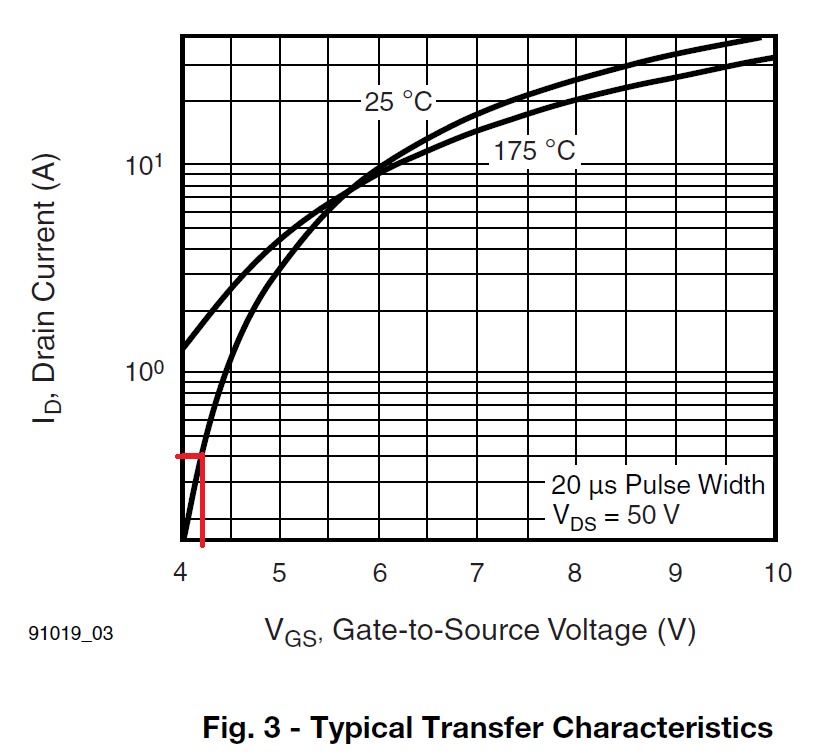
\includegraphics[width=0.5\linewidth]{Imagenes/Punto1/Ej1-VgsIo.png}
\end{figure}

De donde se obtiene:

\[
V_{gsTh} = 4V \hspace{2cm} V_{gsIo} = 4.4V
\]

Cuando el canal no conduce, el valor de $V_{ds} = V2 = 50V$. Con dicho valor se busca en la hoja de datos el valor de la capacidad $C_{gs} + C_{gd1}$, que se encuentra como $C_{iss}$, de la curva $C(V_{ds})$:

\begin{figure}[H]
\centering
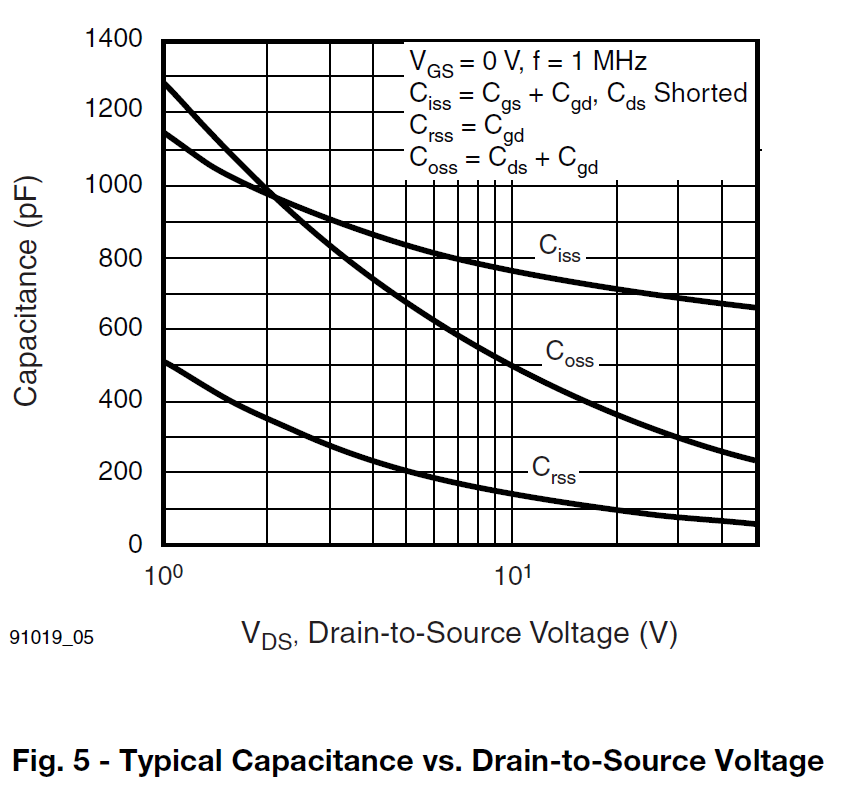
\includegraphics[width=0.5\linewidth]{Imagenes/Punto1/Ej1-Capacidades.png}
\end{figure}

De donde se obtiene que:

\[
C_{gs} + C_{gd1} = 650pF
\]

Con lo que podemos obtener $\tau_1$.

\[
\tau_1 = R_g \cdot (C_{gs} + C_{gd1}) = 65nS
\]

Planteando entonces la curva de $V_{gs}(t)$ para el tramo de encendido hasta que toma el valor de $V_{gsIo}$:

\[
V_{gs} = V_{gg} \cdot (1 - e^{-\frac{t}{\tau_1}})
\]

Despejando $t$, con $V_{gsTh}$ obtenemos el valor de $t_d(ON)$, es decir el tiempo en que tarda en llegar a la tensión de threshold. Y con $V_{gsIo}$ el tiempo en llegar hasta el valor de tensión para la cual el canal puede conducir $I_o$, $t_1 = t_d(ON) + t_{ri}$:

\[
t_d(ON) = -\tau_1 \cdot Ln\left( 1 - \frac{V_{gsTh}}{V_{gg}} \right) = 33,2nS
\]

\[
t_1 = -\tau_1 \cdot Ln\left( 1 - \frac{V_{gsIo}}{V_{gg}} \right) = 37.7nS
\]

Por lo que el valor de $t_{ri}$ (tiempo que tarda el subir $I_d$ hasta llegar a $I_o$) se obtiene por diferencia:

\[
t_{ri} = t_1 - t_d(ON)= 4.5nS
\]

Durante el tiempo que $V_{gs}$ se mantiene constante (que es cuando disminuye el valor de $V_{ds}$), la corriente de Gate ($I_g$) se mantiene constante, debido a la ley de Ohm con la resistencia $R_g$:

\[
I_g = \frac{V_{gg} - V_{gsIo}}{R_g} = 56mA
\] 

Dado que la corriente se mantiene constante, podemos obtener la variación de carga en Gate ($\Delta Q$) durante ese tiempo de la curva $V_{gs}(Q_g)$ provista por la hoja de datos, entrando con el valor de $V_{gsIo}$:

\begin{figure}[H]
\centering
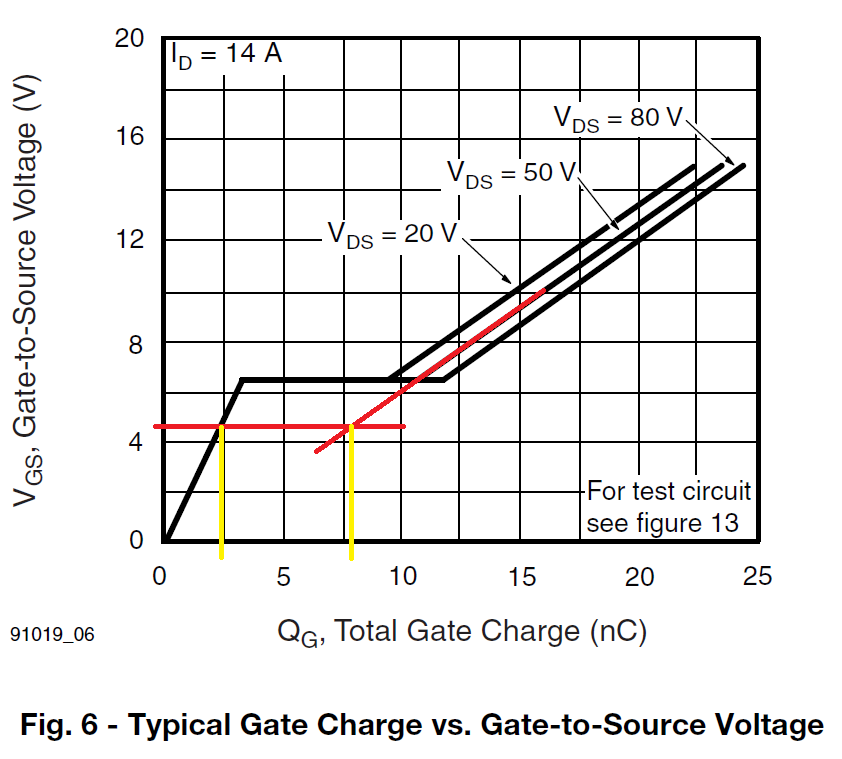
\includegraphics[width=0.5\linewidth]{Imagenes/Punto1/Ej1-GateCharge.png}
\end{figure}

De donde se obtiene que el $\Delta_Q = 6nC$. Sabiendo que la corriente es variación de la carga en el tiempo, podemos despejar el tiempo de caída de $V_{ds}$:

\[
I_g = \frac{\Delta Q}{\Delta t} \Longrightarrow t_{fv} = \frac{\Delta Q}{I_g} = 107nS
\]

\begin{figure}[H]
\centering
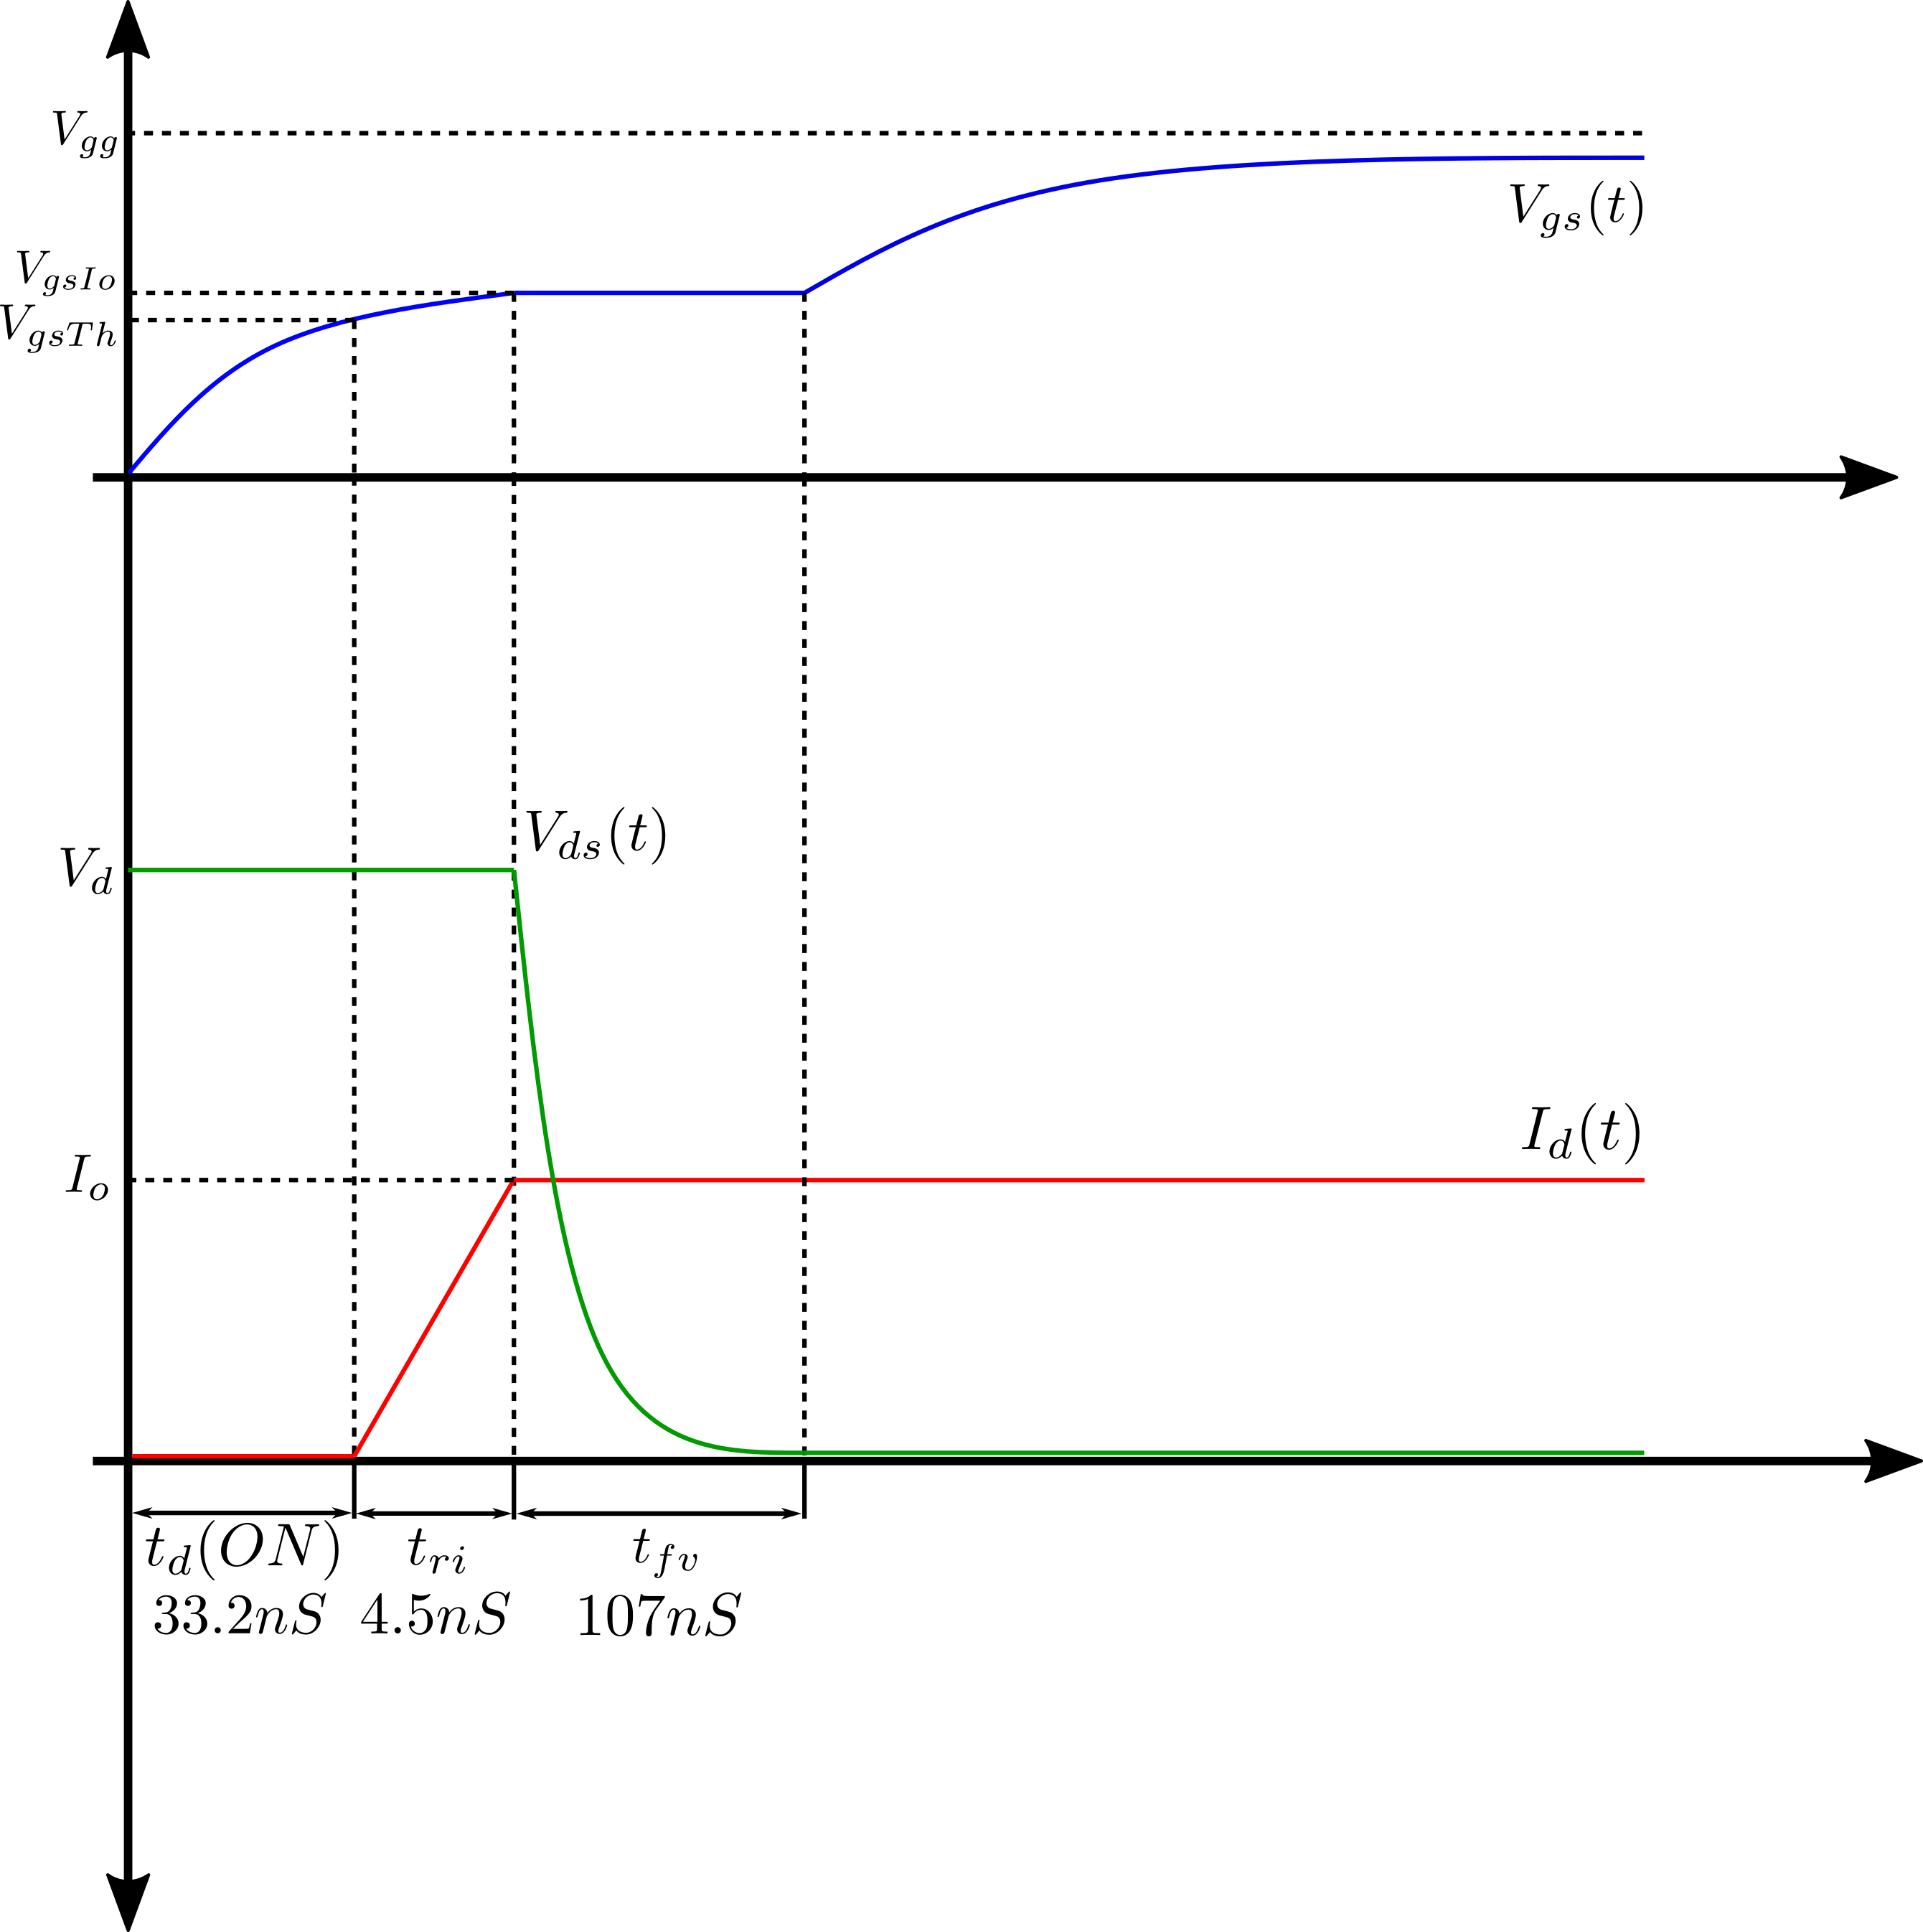
\includegraphics[width=0.8\linewidth]{Imagenes/Punto1/EncendidoTeorico.png}
\caption{Curvas de encendido teórico}
\end{figure}

Cuando el canal conduce $I_o$, el valor de $V_{ds}$ es $V_{ds-ON} = I_d \cdot R_{ds-ON} = 0.8V$. Con esto último, el valor de la capacidad resulta (aproximadamente):

\[
C_{gs} + C_{gd2} = 1150pF
\]

Por lo que podemos obtener $\tau_2$:

\[
\tau_2 = R_g \cdot (C_{gs} + C_{gd2}) = 115nS
\]

Para el apagado, se plantea la curva de $V_{gs}(t)$ para el tramo que va desde el máximo ($V_{gg}$) hasta $V_{gsIo}$, despejando el tiempo que demora, $t_d(OFF)$:

\[
V_{gsIo} = V_{gg} \cdot e^{-\frac{t}{\tau_2}} \Longrightarrow t_d(OFF) = -\tau_2 \cdot ln\left( \frac{V_{gsIo}}{V_{gg}} \right) = 141nS
\]

Para el tiempo que se mantiene $V_{gsIo}$ constante, es cuando aumenta la tensión $V_{ds}$, por lo que usando el valor de $\Delta Q$ hallado previamente se obtiene:

\[
\frac{V_{gsIo}}{R_g} = I_g = 44mA \Longrightarrow t_{rv} = \frac{\Delta Q}{I_g} = 136nS
\]

Y finalmente, el tiempo en que la corriente $I_d$ disminuye, se da entre que $V_{gs}$ pasa de $V_{gsIo}$ a $V_{gsTh}$:

\[
V_{gsTh} = V_{gsIo} \cdot e^{-\frac{t}{\tau_1}}
\]

\[
t_{fi} = -\tau_1 \cdot Ln \left( \frac{V_{gsTh}}{V_{gsIo}}\right) = 6,2nS
\]
 
\begin{figure}[H]
\centering
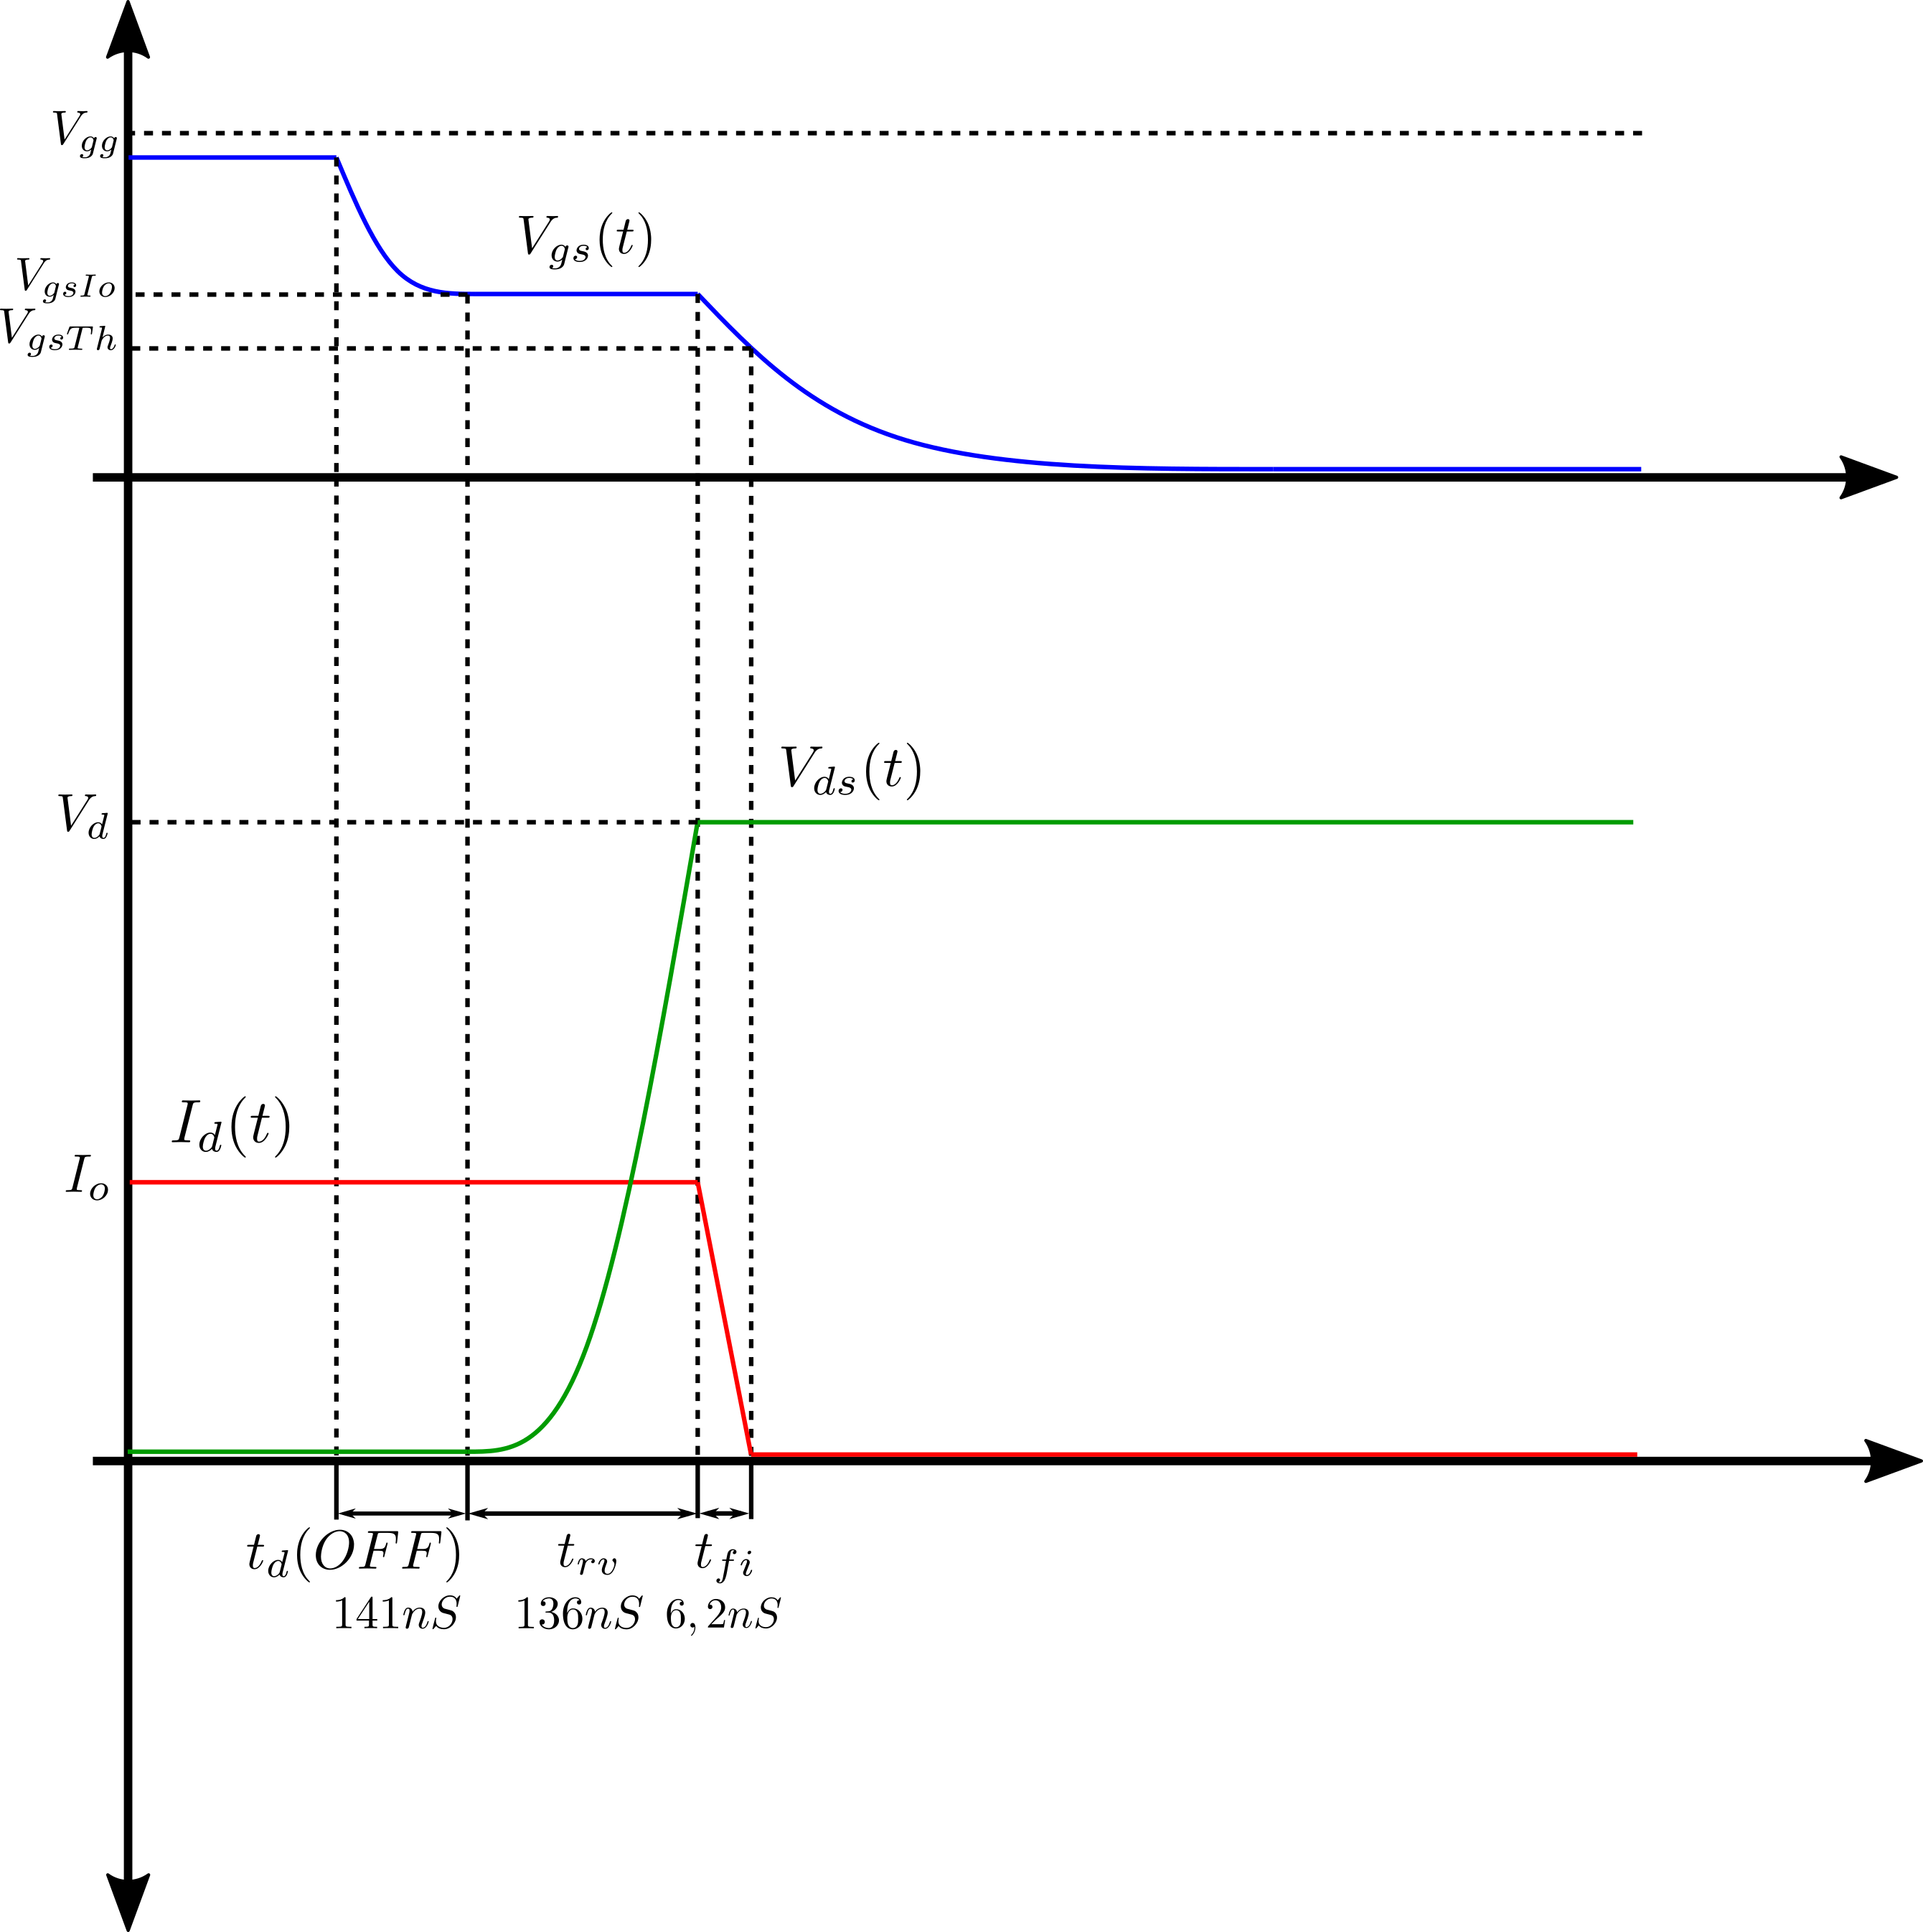
\includegraphics[width=0.8\linewidth]{Imagenes/Punto1/ApagadoTeorico.png}
\caption{Curvas de apagado teórico}
\end{figure}
 
\subsection*{b) Curvas simuladas} 
 
\begin{figure}[H]
\centering
%\includegraphics[width=0.95\linewidth]{Imagenes/Punto1/tiempo_encendido.png}
\caption{Curvas de encendido simulado}
\end{figure}

De donde se tabulan los tiempos:

\[
t_d(ON) = 34nS \hspace{2cm} t_{ri} = 3.72nS \hspace{2cm} t_{fv} = 327nS
\]

\begin{figure}[H]
\centering
%\includegraphics[width=0.95\linewidth]{Imagenes/Punto1/tiempo_apagado.png}
\caption{Curvas de apagado simulado}
\end{figure}

De donde se tabulan los tiempos:

\[
t_d(OFF) = 135.8nS \hspace{2cm} t_{rv} = 523nS \hspace{2cm} t_{fi} = 9.2nS 
\]

\subsection*{c) Comparaciones y observaciones} 
 
\newpage
\end{document}